\documentclass[pdf]{beamer}

\usepackage[utf8]{inputenc}
\usepackage[absolute,overlay]{textpos}
\usepackage{adjustbox}

 
\usetheme{Warsaw}


\mode<presentation>{}
%% preamble

\setbeamercolor{framesource}{fg=gray}
\setbeamerfont{framesource}{size=\tiny}

\newcommand{\source}[1]{\begin{textblock*}{4cm}(8.7cm,8.6cm)
    \begin{beamercolorbox}[ht=0.3cm,right]{framesource}
        \usebeamerfont{framesource}\usebeamercolor[fg]{framesource} Source: {#1}
    \end{beamercolorbox}
\end{textblock*}}


\author{Virgile Audi \\ Nicolas Drizard}
\date{TF: Sam Wiseman \\ May, $3^{rd}$ 2015}
\title{Memory Network For Question Answering}

\begin{document}


%% title frame
\begin{frame}
\titlepage
\end{frame}

\begin{frame}
\frametitle{Outline}
\tableofcontents
\end{frame}

\AtBeginSection[]
{
  \begin{frame}
    \frametitle{Table of Contents}
    \tableofcontents[currentsection]
  \end{frame}
}

\section{Motivation}

\subsection{Questions}
\begin{frame}{Supporting Facts}

\textbf{Story} 
\begin{center}
Mary went to the bathroom.\\
John moved to the hallway.\\
Mary travelled to the office.
\end{center}

\textbf{Q} Where is Mary? \textbf{A} office

\textbf{Story} 
\begin{center}
John picked up the apple.\\
John went to the office.\\
John went to the kitchen.\\
John dropped the apple.
\end{center}

\textbf{Q} Where was the apple before the kitchen? \textbf{A} office
\end{frame}

\begin{frame}{Reasoning}

\textbf{Story} 
\begin{center}
Sheep are afraid of wolves.\\
Cats are afraid of dogs.\\
Mice are afraid of cats.\\
Gertrude is a sheep.
\end{center}

\textbf{Q} What is Gertrude afraid of? \textbf{A} wolves

\textbf{Story}
\begin{center}
Lily is a swan.\\
Lily is white.\\
Bernhard is green.\\
Greg is a swan.
\end{center}

\textbf{Q} What color is Greg? \textbf{A} white
\end{frame}

\subsection{Intuition}

\begin{frame}{Intuition}

How do Humans build their answer?

\begin{enumerate}
	\item Type of question
	\item Occurence of the words from the question
	\item Associations of words (\textit{memory})
	\item Meaning of words (\textit{reasoning}, \textit{interpretation})
\end{enumerate}

\end{frame}

\section{Baseline Model}

\begin{frame}{Count Based Model}

Prediction based on two features:

\[
\hat{y}(X,Q) = argmax(\log(f_1(X)) + \log(f_2(Q)))
\]

with 

\begin{itemize}
	\item $(X, Q)$ tuple story, question
	\item $f_1(X)$: answer words counts in the story (weighted by order of appearance)
	\item $f_2(Q)$: embedding of the question based on possible answers question word
\end{itemize}

\end{frame}

\section{End-to-end Memory Network}
\subsection{Architecture}

\begin{frame}{Single Hop Architecture}
\begin{figure}
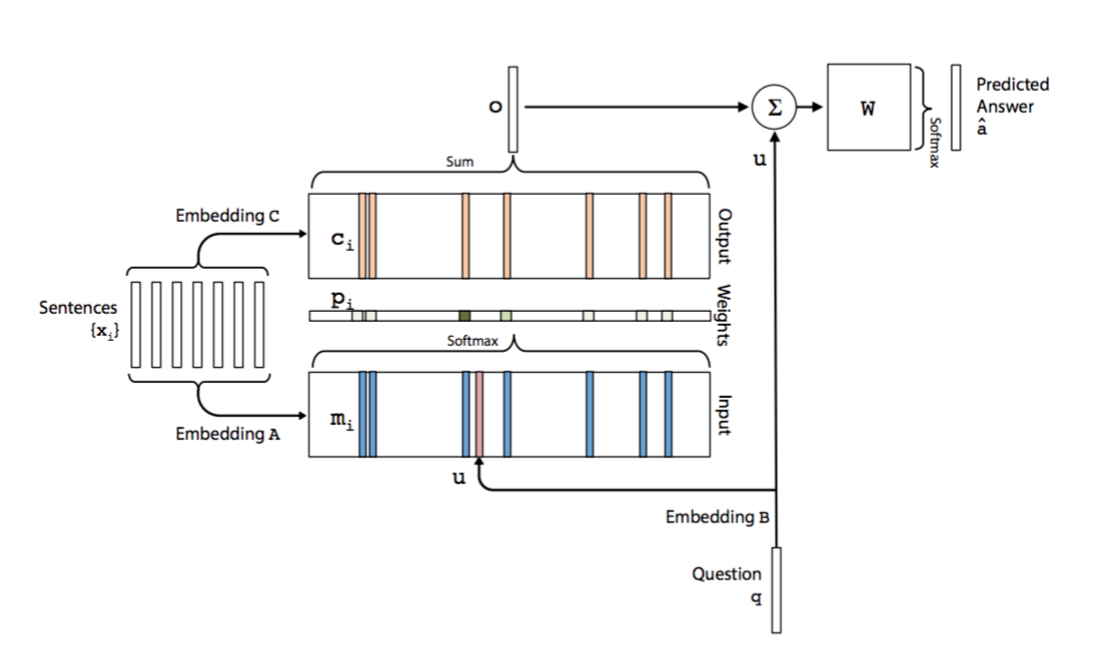
\includegraphics[scale=0.45]{mem.png}
\caption{Single Hop architecture}
\source{End-To-end Memory Networks}
\end{figure}
\end{frame}

\begin{frame}{Multiple Hops Architecture}
\begin{figure}
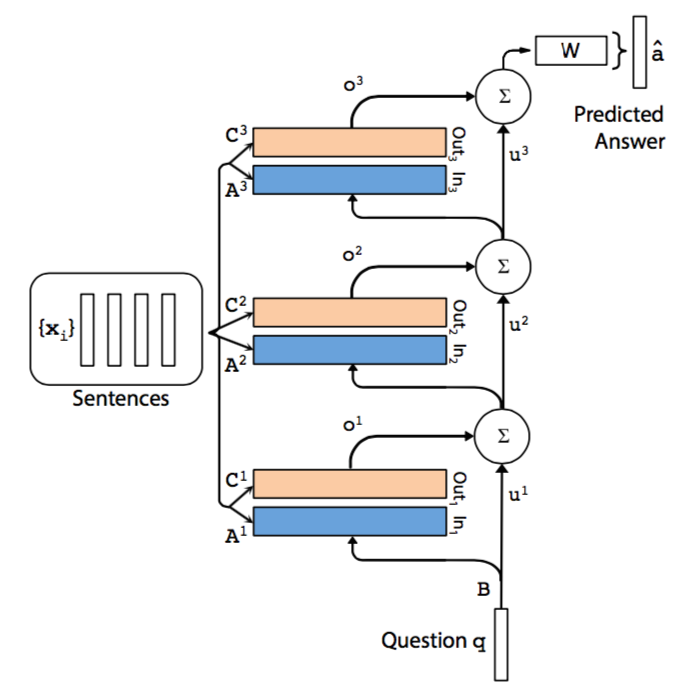
\includegraphics[scale=0.45]{mem_multiple.png}
\caption{Multiple Hops architecture}
\source{End-To-end Memory Networks}
\end{figure}
\end{frame}

\subsection{Parameters Tying}

\begin{frame}{Parameters Tying}
Two Approaches to reduce the number of parameters:

\begin{itemize}
	\item \textbf{Adjacent}
		\begin{itemize}
			\item $A^{k+1} = C^{k}$
			\item $B = A^1$
		\end{itemize}
	\item \textbf{RNN-like}
		\begin{itemize}
			\item $A^1 = A^2 = ... = A^k$
			\item $C^1 = C^2 = ... = C^k$
			\item $u^{k+1} = Hu^k + o^k$
		\end{itemize}
\end{itemize}

\end{frame}

\subsection{Implementation Details}

\begin{frame}{Implementation Tricks}
\begin{itemize}
	\item bag-of-words representation $x_i = \{x_{i1}, ..., x_{is}\}$ becomes $m_i = \sum_j Ax_{ij}$
	\item Temporal encoding $m_i = \sum_j Ax_{ij} + T_A(i)$
	\item high variance, best model over several training
\end{itemize}	
\end{frame}

\section{Result}

\begin{frame}{Train Results}
\begin{table}[]
\centering
\label{my-label}
\adjustbox{max height=\dimexpr\textheight-4.7cm\relax,
           max width=\textwidth}{
           \begin{tabular}{|l|l|l|l|}
\hline
Task                     & \begin{tabular}[c]{@{}l@{}}MemNN 1 hop\\ adjacent\end{tabular} & \begin{tabular}[c]{@{}l@{}}MemNN 3 hops\\ adjacent\end{tabular} & Baseline \\ \hline
1: 1 supporting fact     & 100                                                            & 99                                                              & 50       \\ \hline
2: 2 supporting facts    & 16                                                             & 90                                                              & 40       \\ \hline
3: 3 supporting facts    & 25                                                             & 85                                                              & 26       \\ \hline
4: Two arg relation      & 71                                                             & 79                                                              & 34       \\ \hline
5: Three arg relation    & 86                                                             & 89                                                              & 48       \\ \hline
6: Yes/No                & 51                                                             & 97                                                              & 50       \\ \hline
7: Counting              & 87                                                             & 80                                                              & 49       \\ \hline
8: Lists/Sets            & 90                                                             & 90                                                              & 0        \\ \hline
9: Simple Negation       & 64                                                             & 86                                                              & 64       \\ \hline
10: Indefinite Knowledge & 61                                                             & 85                                                              & 44       \\ \hline
11: Basic coreference    & 80                                                             & 87                                                              & 63       \\ \hline
12: Conjunction          & 100                                                            & 100                                                             & 60       \\ \hline
13: Compound Coref       & 93                                                             & 93                                                              & 68       \\ \hline
14: Time Reasoning       & 72                                                             & 94                                                              & 29       \\ \hline
15: Basic Deduction      & 39                                                             & 39                                                              & 14       \\ \hline
16: Basic Induction      & 50                                                             & 54                                                              & 52       \\ \hline
17: Size Reasoning       & 53                                                             & 62                                                              & 48       \\ \hline
18: Positional Reasoning & 61                                                             & 63                                                              & 53       \\ \hline
19: Path Finding         & 24                                                             & 24                                                              & 0        \\ \hline
20: Agent's Motivation   & 92                                                             & 92                                                              & 52       \\ \hline
\textbf{TOTAL}           & \textbf{66}                                                    & \textbf{82}                                                     &          \\ \hline
\end{tabular}
}
\end{table}
\end{frame}


\section{Future Steps}

\begin{frame}
\begin{itemize}
	\item Positional Encoding
	\item MC Test dataset
	\item Dynamic Memory
\end{itemize}
\end{frame}




\end{document}